
\chapter{Úvod}

V minulých letech na Fakultě Informačních Technologií VUT v Brně vznikl výukový simulátor superskalárního procesoru pro potřeby předmětu Architektury výpočetních systémů.
Simulátor v současné době slouží jako interaktivní a názorná ukázka probíraných principů. 

V této práci navážu na předchozí úsilí a pokusím se vylepšit dostupnost a přesnost simulátoru.
Mým cílem je vylepšit rozhraní simulátoru, konkrétně vyvinout webovou aplikaci a rozhraní pro příkazovou řádku.
Od nových rozhraní očekávám lepší názornost a tedy vetší užitek pro výuku.

V první části práce se zaměřím na principy, na kterých jsou moderní superskalární procesory založeny, především na ty, které jsou v simulátoru demonstrovány.
Prozkoumám i metody tvorby webových aplikací a jejich nasazení do provozu.

Následně zanalyzuji dosavadní řešení a navrhnu jejich vylepšení a rozšíření.

V poslední části práce popíšu implementaci a zhodnotím přínos pro výuku.

%
% Superskalární procesory
%

\chapter{Skalární procesor}
% pohled programátora a pohled HW
% jak se zvyšuje výkon
% funkční jednotky
% 
% superskalár
% konflikty
% algoritmy tomasulo

Jádro procesoru představuje centrální prvek CPU, který provádí výpočet popsaný instrukcemi určité instrukční sady.
Z abstraktního pohledu se procesor nachází v definovaném stavu a vykonáním každé instrukce se dostává do následujícího stavu.
Tento stav je představován hodnotami v registrech.
Společně se stavem hlavní paměti tvoří stav výpočtu.
Instrukční sada tvoří \emph{programátorův model CPU}.

Programátorův model CPU je abstraktní reprezentace funkcionality a chování procesoru.
Je navržena tak, aby usnadnila programátorův proces psaní kódu.
Příklady instrukční sady jsou RISC-V, nebo Intel 64.

Instrukční sada nepopisuje jak má vypadat implementace procesoru, ale pouze popisuje \emph{prostředí a zdroje}, které program může využít.
Této volnosti využívají implementace, které mohou zpracovávat více instrukcí současně, i mimo původní pořadí programu, případně i spekulativně.
Návrháři instrukční \cite{QuantApproach}

V této kapitole popíšu různé techniky využívané v efektivních implementacích jader procesorů.
Krátce se budu věnovat skalárním procesorům, ale většina kapitoly se bude věnovat přímo superskalárním procesorům.

\section{Složky výpočetního jádra}
% https://www.cise.ufl.edu/~mssz/CompOrg/CDA-proc.html

Instrukční sada definuje počet instrukcí nutných k určitému výpočtu, implementace procesoru ale rozhoduje o jeho celkovém výkonu.

Jednoduchá implementace dělí datovou cestu do následujících stádií:
\begin{enumerate}
    \item \emph{Fetch} -- Načtení instrukce,
    \item \emph{Decode} -- Dekódování instrukce, čtení registrů,
    \item \emph{Execute} -- Vykonání samotného výpočtu,
    \item \emph{Memory Access} -- Přístup k paměti,
    \item \emph{Write Back} -- Zápis do registrů (propsání stavu procesoru).
\end{enumerate}
Tato datová cesta je prováděna během jednoho cyklu.
Stádia mohou sdílet hardware.
Ne každá instrukce potřebuje všechny stádia, například uložení do paměti nemá poslední fázi zápisu do registru.

Tato stádia jsou vhodně zvolena, jejich provedení může být nezávislé.
Jejich nezávislost dovoluje vydělit pro každou část speciální hardware a jejich výpočet \emph{paralelizovat}.
Vznikne řetězená linka.
\cite{OrganizationAndDesign}

Bez řetězení by se musel zvolit takt procesoru podle nejpomalejší instrukce. 

\subsection{Fáze výpočtu}
% https://en.wikipedia.org/wiki/Classic_RISC_pipeline

Následuje detailnější popis fází klasické pětistupňové linky.

\subsubsection{Instruction Fetch (IF)}

Prvním krokem zpracování instrukce je její načtení z paměti.
Z paměťového modulu je načtena instrukce na adrese uložené v registru \texttt{PC}.
Implementace mají pro tento účel dedikovanou vyrovnávací paměť a jednotku přednačítání, které zajišťují, že tato fáze proběhne v jednom cyklu.

Registr \texttt{PC} je ovlivňován skokovými instrukcemi.
Jejich výsledky jsou ale známy až v pozdějších fázích linky.
Proto jednotka fetch v taktech, kdy není známa adresa následující instrukce, vkládá do linky prázdné instrukce (\texttt{nop}, nebo také \emph{bubbles}).

Jedním způsobem, jak na výpočet skoku nemuset čekat, je skok \emph{předpovědět}.
Tento koncept bude rozveden v sekci \ref{branchpredict}.

\subsubsection{Instruction Decode (ID)}

Během této fáze jsou dekódovány binární instrukce a převedeny na interní kódy, které CPU může vykonat.
Tato fáze také zahrnuje identifikaci operačního kódu a přiřazení a načtení příslušných registru a operandů k provedení dané instrukce.

Při zpracovávání skokových instrukcí se zároveň se čtením počítá cílová adresa skoku.
Podmínka je vypočtena ve fázi execute, čímž v případě, že se skok má uskutečnit, vznikne pokuta 1 cyklus.

U procesorů se zpracováním mimo pořadí zde dojde k přejmenování registrů.
Architektury CISC v této fázi dekódují instrukci na jednu nebo více mikroinstrukcí.
Dále zpracovávají mikroinstrukce.

\subsubsection{Execute (EX)}

Ve fázi execute dochází k provedení výpočtu instrukce.
Hardware zahrnuje ALU, posuvný registr, násobičku a děličku.
Výpočet probíhá nad daty načtenými ve fázi ID.

Paměťové instrukce zde vypočítají adresu pro přístup do paměti. 

Délka fáze execute se může mezi instrukcemi významně lišit.
Tabulka \ref{table:ex_latency} ukazuje několik instrukcí implementace Intel Ice Lake instrukční sady x86.
% todo jak se to řeší v lince?

\begin{table}[ht]
\centering
\caption{Vybrané instrukce a jejich latence v cyklech architektury Intel Ice Lake. Předpokládá se, že neproběhnou přístupy do paměti nevzniknou výjimky. \cite{instructionTables}}
\begin{tabular}{|l|l|l|}
\hline
Instrukce & Latence (cykly) & Popis                                                          \\ \hline\hline
MOV r, r  & 1       & Kopie hodnoty mezi registry                                    \\ \hline
CMP r, r  & 1       & Porovnání hodnot, nastavení příznaků                           \\ \hline
ADD (32b) & 1       & Součet dvou hodnot v registrech (šířka 32 bitů)                \\ \hline
MUL (32b) & 4       & Násobení dvou hodnot v registrech (šířka 32 bitů)              \\ \hline
DIV (32b) & 12      & Dělení dvou hodnot v registrech (šířka 32 bitů)                \\ \hline
FMUL      & 4       & Násobení dvou hodnot v registrech (float 32 bitů)   \\ \hline
FSIN      & 60-120  & Výpočet funkce $sin(x)$                                        \\ \hline
\end{tabular}
\label{table:ex_latency}
% https://www.agner.org/optimize/instruction_tables.pdf
% strana 348
\end{table}

\subsubsection{Memory Access (MA)}

Fáze "memory access" v CPU zahrnuje přístup k paměti pro čtení nebo zápis dat.
Využívá k němu adresu, která byla dříve vypočtena ve fázi execute.
Instrukce, které nepřistupují k paměti v této fázi neprovádí žádnou operaci.

Zápisy do paměti jsou nejdříve provedeny pouze do dočasného registru, aby mohly být v případě výjimky anulovány.

Pokud proces pracuje v režimu s \emph{virtuálním adresovým prostorem}, je nutné virtuální adresu přeložit na fyzickou adresu.
K překladu slouží hardwarové jednoty PT walker a Translation Lookaside Buffer (TLB).

Délka přístupu do hlavní paměti (DRAM) může trvat přibližně 100 nanosekund, tedy 100 taktů při frekvenci 1 GHz.
Pokud by všechny přístupy do paměti byly vyřízeny v hlavní paměti, čas přístupu do paměti by dominoval výpočtu.
Za účelem zkrácení doby přístupu procesor k paměti přistupuje skrze systém \emph{cache}.
Cache kopíruje část hodnot z hlavní paměti do paměti s významně kratší dobou přístupu, čímž zajišťuje, že fáze MA může být provedena v rámci cyklu.
Pokud hodnota v cache není, je nutné celou linku zastavit.
Detailnější popis vyrovnávací paměti je uveden v sekci \ref{cache}.

\subsubsection{Write Back (WB)}

V této fázi dochází k zápisu výsledku instrukce do registrů.
K registrům v rámci cyklu přistupuje i hardware fáze decode.
Tento strukturní konflikt musí být vyřešen.

Jsou zde řešeny výjimky, které jsou do této fáze propagovány.
Výjimka je obsloužena ve dvou krocích: (1) linka je vypláchnuta a (2) PC je nastaven na adresu procedury, která výjimku ošetřuje.

\subsection{Řetězená linka}

Řetězení je formou časového paralelismu.
Více instrukcí postupuje jednotlivými stupni linky najednou, čímž zvyšují vytížení a propustnost procesoru.
Jednotlivé stupně jsou spojeny za sebou, mezi každými dvěma stupni se nacházejí registry pro předání dat.
Rozdělením zpracování každého z $n$ kroků do speciální hardwarové stanice je možné v procesoru vytvořit \emph{řetězenou linku} (\emph{pipeline}) hloubky $n$.
Maximální možné zrychlení linky odpovídá hloubce linky.
Ideálně v každém taktu procesor opouští jedna instrukce a $IPC = 1$ (IPC -- instruction per clock).

Pro dosažení maximálního zrychlení je nutné zajistit nepřetržitý přísun nezávislého kódu ke zpracování a stejnou dobu výpočtu každého stupně.
Pokud výpočty stupňů nejsou stejně dlouhé, je nutné jako čas cyklu zvolit nejdelší z nich.
Náběh a doběh linky a zpoždění registrů mezi jednotlivými stupni se při výpočtu zrychlení zanedbávají.

Kromě výše uvedených komplikací je v realitě propustnost snižována zastavováním linky (\emph{stall}).
Důvodem zastavování linky jsou \emph{konflikty}. \cite{OrganizationAndDesign}

\subsubsection{Konflikty}

Mezi dvojicí instrukcí dochází k datovému konfliktu, když jedna instrukce provádí výpočet nad daty generovanými druhou instrukcí.
Tuto situaci označujeme \emph{read after write} (RAW).
K předání dat dochází prostřednictvím registrů nebo hlavní paměti.
Tato závislost může při paralelizaci ve zřetězené lince způsobit chybný výpočet.
Stát se tak může, pokud druhá instrukce začne výpočet dříve, než ho první instrukce zpřístupní.

Řešením konfliktu je pozdržení výpočtu dokud výsledek instrukce není k dispozici.
Obrázek \ref{dataconflictsfrombook} ilustruje situaci, při které se musí linka zastavit pro zachování správnosti výpočtu.
Konflikty mohou být částečně kompenzovány vhodným návrhem programu, respektive překladačem, který kód přeuspořádá tak, aby maximálně vykryl čekání na konflikty užitečnou prací.
% todo detekce a forwarding

Pokročilejším řešením je předávání dat mezi fázemi linky speciálními cestami, takzvanými zkratkami.
Zkratky mohou eliminovat potřebu zastavovat linku, čímž zvýší její propustnost.

\begin{figure}[ht]\centering
  \centering
  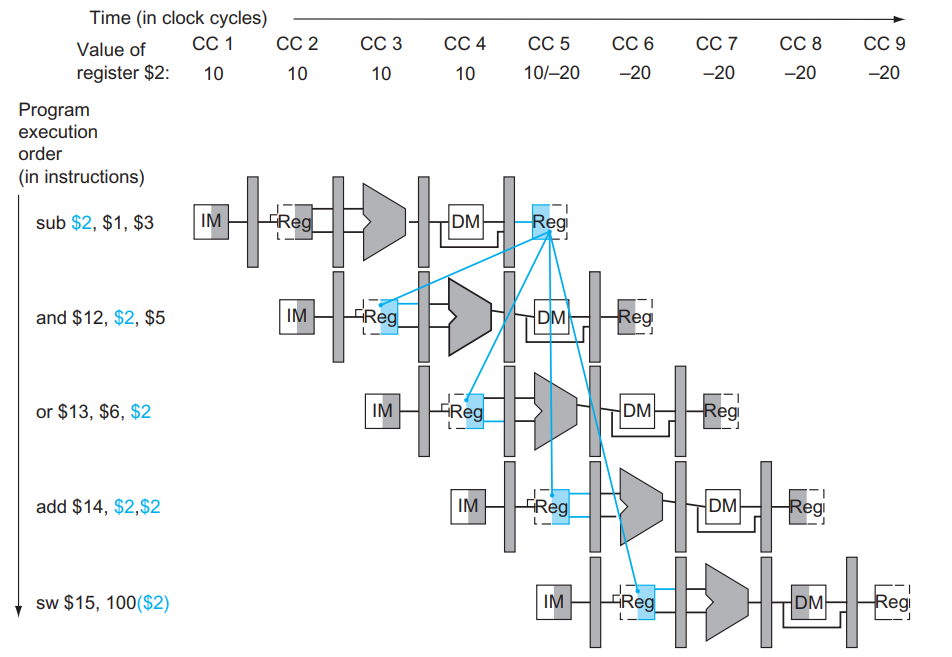
\includegraphics[width=15cm]{obrazky-figures/conflicts.png}
  \caption{Sekvence instrukcí vykonávaných ve skalární lince.
  Zvýrazněné závislosti mezi registry ukazují, že hodnota \texttt{\$2} čtená instrukcí \texttt{and} není výsledkem předchozí instrukce. \cite{OrganizationAndDesign}}
  \label{dataconflictsfrombook}
\end{figure}

\subsection{Další části procesoru}
% brány, registrové pole, hlavní paměť
% TLB? stránky?
% přerušení a jádro?
% Další jádra a jejich spojení

Byly zmíněny hlavní komponenty procesoru, ty ale nemohou pracovat izolovaně.
V jádře se především nachází řídící logika (control unit).
Tato jednotka pomocí signálů ovládá datovou cestu, paměťová a vstupně-výstupní zařízení.
Jednoduchá řídící logika může být implementována jako konečné stavové řízení.
\cite{OrganizationAndDesign}

Modul Memory Access bývá napojen na hlavní paměť, cache a tabulku stránek.
Write Back je napojen na registrové pole.

Další části jádra procesoru slouží k optimalizaci těchto základních funkcí.
Prediktory budou probrány v sekci \ref{branchpredict}.

\section{Vyrovnávací paměť}
\label{cache}
% todo

Paměť, která je dostatečně rychlá pro současné procesory, je zároveň velmi drahá.
Řešením tohoto problému je \emph{hierarchie pamětí} -- víceúrovňová struktura, kde úrovně blíž procesoru mají menší kapacitu, ale větší rychlost.
Výsledkem je vyvážený stav mezi výkonem a cenou.

Hierarchie pamětí funguje dobře, protože přístupy do paměti nebývají zcela náhodné, ale řídí se \emph{principem lokality}.
Prvním typem lokality je časová lokalita.
Ta tvrdí, že k paměťovým místům, ke kterým bylo přistoupeno nedávno, bude pravděpodobně v blízké době přistoupeno znovu.

Druhým typem lokality je prostorová lokalita.
Ta předvídá, že k fyzicky blízkým paměťovým místům se přistupuje blízko v čase.

Pokud programy tyto principy při práci s pamětí dodržují, mají tendenci vykazovat lepší výkon.
\cite{QuantApproach}

Hierarchie pamětí na nejrychlejší úrovni využívá registry.
Na další úrovni je vyrovnávací paměť (cache), poslední úroveň tvoří hlavní paměť.
Modely s více úrovněmi cache jsou běžné, k popsání základních principů se ale budu věnovat modelu s jednou úrovní cache.
Programátor s pamětí pracuje jako s celkem, hierarchie pamětí se projevuje pouze rychlostí výpočtu.

Cache obsahuje části hlavní paměti (bloky) se kterými procesor momentálně pracuje.
Nové bloky jsou alokovány při čtení nebo zápisu na paměťové místo, které se v cache momentálně nenachází.
Záznam v cache obsahuje informaci o původní lokaci bloku v paměťovém prostoru, aby později mohl být vrácen do hlavní paměti.
Bloky jsou v paměti zarovnané na násobek své velikosti.

Nejčastěji používaná strategie ukládání bloků je \emph{asociativní cache}.
Úložiště pro bloky je v této variantě rozděleno do skupin o $m$ blocích.
Každý blok hlavní paměti je částí své adresy (indexem) mapován na právě jednu skupinu.

Zajímavé jsou krajní případy.
Pokud $m = 1$, potom se cache nazývá přímo mapovaná.
Pokud $m$ odpovídá kapacitě cache, potom se cache nazývá plně asociativní.

Pokud ve skupině není pro nový blok místo, je nutné jeden blok vybrat, přemístit ho zpět do hlavní paměti a tím místo uvolnit.
Nejznámější strategie výběru bloku ve skupině (victim) jsou:
\begin{itemize}
    \item náhodný výběr,
    \item FIFO (výběr nejstaršího bloku),
    \item LRU (nejdéle nepoužitý blok).
\end{itemize}
Efektivita cache se vyjadřuje četností nalezení požadovaného bloku (hit rate) v procentech.

Hledání bloku ve skupině je prováděno paralelním porovnáním jiné části adresy (tagu).
Použití částí adresy je naznačeno na obrázku \ref{cachelineaddress}.

\begin{figure}[ht]\centering
  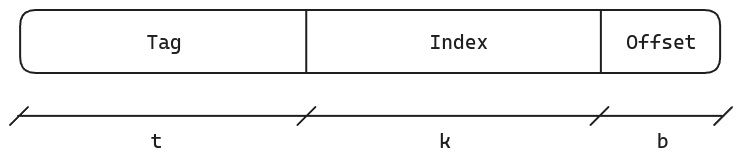
\includegraphics[width=11cm]{obrazky-figures/cacheline.png}
  \caption{Adresa paměti a její části. Prvních \texttt{t} bitů je použito jako \emph{tag} k vyhledání v rámci skupiny. Následujících \texttt{k} bitů adresuje skupinu a posledních \texttt{b} bitů adresuje obsah bloku.}
  \label{cachelineaddress}
\end{figure}

% todo víceúrovňová cache

\chapter{Superskalární procesor}
% multiple issue
% https://en.wikipedia.org/wiki/Superscalar_processor

% e performance of a computer is determined by three key
% factors: instruction count, clock cycle time, and clock cycles per instruction (CPI).
Délka výpočtu je určena třemi hlavními faktory: počtem instrukcí, frekvencí hodinového signálu a počtem instrukcí provedených za hodinový signál (\emph{Instructions Per Clock -- IPC}).
Architektura superskalárních procesorů zvyšuje výkon zvýšením IPC, typicky až nad hodnotu 1 -- jinými slovy, mohou vykonat 2 a více instrukcí ve stejný čas. \cite{QuantApproach}

Superskalární procesory rozšiřují řetězení na úrovni instrukcí ze skalárních řetězených procesorů.
K časovému paralelismu přidávají \emph{prostorový paralelismus}, který spočívá v rozšíření linky na $m$ instrukcí v každém stupni a duplikací potřebných hardwarových jednotek.
Výsledkem je, že superskalární procesory mohou \emph{vydat} k výpočtu více instrukcí v jednom taktu.
Cenou za zrychlení je zvýšení složitosti obvodu a tím nižší dosažitelný kmitočet, vyšší spotřeba energie a větší plocha čipu.

Existuje velké množství technik sloužících ke snižování doby zastavení linky.
V této kapitole je blíže rozvedeno dynamické plánování, provádění kódu spekulativně a mimo pořadí.
Tyto koncepty bývají vysvětlovány a implementovány zároveň, pokusím se je ale vysvětlit izolovaně.
Zmíněné metody jsou pouze výběrem z možných způsobů implementace superskalárních procesorů.

% in order superscalar
% scoreboarding??

\section{Konflikty}
\label{conflicts}

Kapitola o skalárních procesorech definovala konflikt jako datovou závislost mezi dvěma instrukcemi.
Pro superskalární procesory je užitečné tento problém rozvést blíže.

V případě, kdy dochází k přeuspořádání pořadí vykonání instrukcí, je nutné uvažovat i \emph{nepravé} datové konflikty.
Pořadí pravých datových konfliktů (RAW) musí být respektováno, protože na rozdíl od nepravých nesou význam výpočtu. Jinými slovy nelze prohodit pořadí vykonání instrukcí s pravým datovým konfliktem.

Nepravé konflikty můžeme charakterizovat jako konflikty jmen.
Vznikají znovupoužitím jména paměťového místa v důsledku konečného počtu registrů, nebo vícenásobným vykonáním stejné instrukce.
Důležité je, že nepravou závislost lze na rozdíl od pravé závislosti odstranit bez ovlivnění správnosti výpočtu, protože mezi instrukcemi nejsou vyměňována žádná data.
Nepravé závislosti lze řešit přejmenováním při tvorbě programu (programátorem nebo překladačem), nebo za běhu řídícím hardwarem procesoru.
Algoritmy Scoreboarding a Tomasulo, které jsou při řešení konfliktů využívány, uvedu v sekci \ref{chap:ooo}.

Obrázek \ref{dataconflicts} vizualizuje pravé i nepravé konflikty mezi registry.

\begin{figure}[ht]\centering
    % add a2, a0, a1
    % mul a3, a2, a1
    % sub a1, a0, a4
    % xor a3, a5, a6
  \centering
  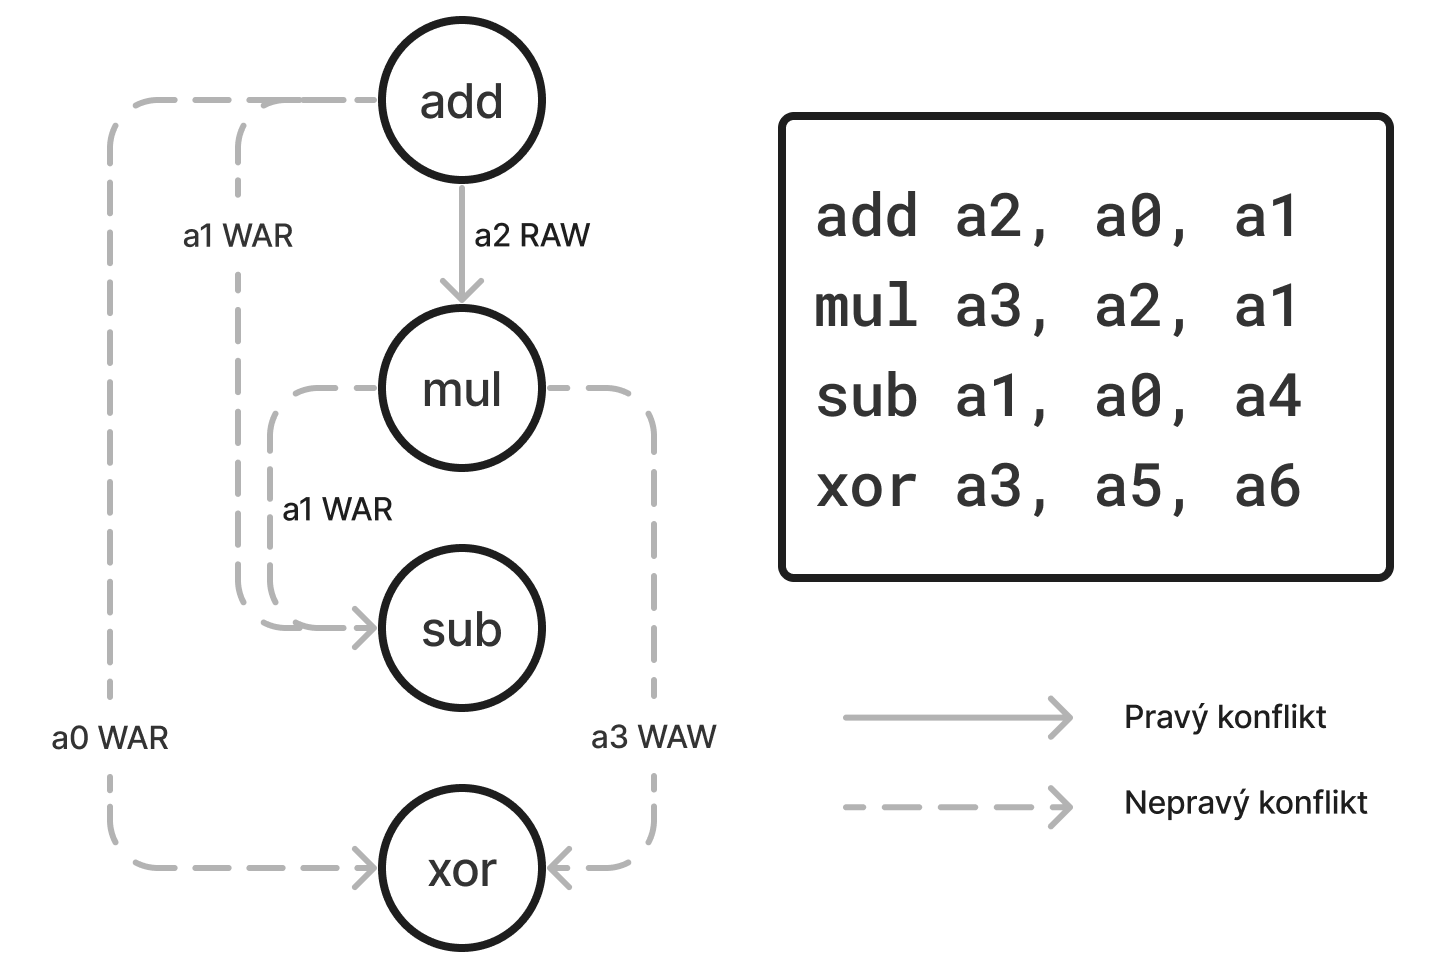
\includegraphics[width=13cm]{obrazky-figures/dataconflicts.png}
  \caption{Program a jeho datové závislosti zobrazené jako graf. Nepravé konflikty jsou zobrazeny přerušovanou čarou, pravé konflikty plnou čarou. Jediná pravá závislost je mezi instrukcemi \texttt{add} a \texttt{mul}, ostatní dvojice instrukcí mohou být vykonány v libovolném pořadí (za předpokladu přejmenování registrů).}
  \label{dataconflicts}
\end{figure}

\subsection{Řídící konflikty}

Skokové instrukce manipulují programový čítač (PC).
Důsledkem je, že pořadí vykonání instrukcí je známo až při samotném výpočtu.
Adresa následující instrukce není při zřetězeném zpracování známa po prvním stupni linky (procesor nezná ani typ zpracovávané instrukce, dokud není dekódována), procesor tedy typicky předpokládá, že instrukce skoková není a začíná zpracovávat následující instrukci.

Pokud dojde ke zpracovávání nesprávné instrukce, musí být z linky odstraněna.

Linka je zastavena, dokud není vypočítána adresa následující instrukce, proto je žádoucí tento výpočet urychlit.
Techniky pro eliminaci pokut skokových instrukcí zahrnují predikci skoků a předsazení výpočtu podmínky v lince.

\subsection{Strukturní konflikty}

Ke strukturnímu konfliktu dochází, pokud vykonání dvou instrukcí vyžaduje stejný prostředek.
Prostředkem je myšlen hardwarový modul, například funkční jednotka, zápisová brána.

Tento typ konfliktu se řeší serializací zpracování, neboli čekáním.
Dopady konfliktů se zmenšují znásobením hardwaru, například přidáním více aritmetických jednotek (ALU).

\section{Zpracování instrukcí mimo pořadí}
\label{chap:ooo}
% https://stackoverflow.com/questions/10074831/what-is-general-difference-between-superscalar-and-out-of-order-ooo-execution
% https://stackoverflow.com/questions/49601910/out-of-order-execution-vs-speculative-execution

Většina procesorů se zpracováním mimo pořadí jsou zároveň superskalární, ale nemusí být nutně.
Tento koncept uvádím v kapitole o superskalárních procesorech, protože jsou to úzce spojené koncepty.

Během výpočtu musí být zachována platnost programovacího modelu, který říká, že projevy instrukcí musí být aplikovány v pořadí.
Zpracování instrukcí mimo pořadí dovoluje provádět práci na jiných instrukcích, než ta, která je právě v pomyslné lince na řadě, aniž by model porušila.
Instrukce nemohou být vykonávány v libovolném pořadí, algoritmus musí instrukci označit jako připravenou k vykonání.
Analýza závislostí spočívá v detekci datových konfliktů registrů tak, jak je popsána v předešlé sekci \ref{conflicts}.
Komplikace nastává u paměťových operací -- konflikty RAW, WAW a WAR nelze odhalit analýzou závislostí registrů, protože konflikty vznikají v hlavní paměti a mohou být ověřeny až jsou vypočítány adresy. 

% limited OOO - předbíhání jen některého druhu (load before load)
Aby byla dodržena sémantika programu a zároveň bylo umožněno vykonávat paměťové instrukce mimo pořadí, je v procesorech zaveden koncept \emph{relaxované paměťové konzistence}.
Čtení a zápisy se mohou přeuspořádat, pokud není narušena správnost programu.
Pokud je z nějakého důvodu nutné vynutit pořadí paměťových operací, je nutné vložit explicitní bariéry.
Paměťové instrukce za bariérou se začnou vykonávat až jakmile jsou všechny paměťové instrukce před bariérou dokončeny.
% release, acquire, ...

Linka procesoru se dělí na dvě části. 
Front-end superskalárního procesoru odpovídá stupňům Instruction Fetch (IF) a Instruction Decode (ID).
Back-end odpovídá stupňům Execute (EX), Memory Access (MA) a Write Back (WB).
Front-end pracuje v pořadí programu.
Back-end pracuje mimo pořadí programu (OOO -- out of order), instrukce back-end opouští opět v původním pořadí.
V rámci back-endu se mohou libovolně promísit přístupy do paměti a vykonávání všech instrukcí v okně. Stále ale musí být respektovány datové závislosti.

% fáze vydání nebo potvrzení?
V cyklu zpracování instrukce přibývá fáze vydání instrukce (\emph{instruction commit}).
Vydání proběhne jakmile je instrukce na řadě a výsledek je vypočítán.
Výsledkem vydání je propsání do vnějšího stavu procesoru.

Procesor identifikuje nezávislé instrukce a vykoná je paralelně.
Tím snižuje počet zastavení linky a zvyšuje IPC.

Skokové instrukce představují asi 20\% instrukcí programu.
Z toho vyplývá, že okno instrukcí, o kterých víme, že budou vykonány, je příliš malé.
Proto bývá zpracování mimo pořadí nejčastěji spojeno se spekulativním vykonáváním. 

% todo komplikace se závislostmi v hlavní paměti
% mělo by to být zde, v konfliktech, nebo v spekulaci?

\subsection{Reorder Buffer}

Pokud jsou instrukce vykonávány mimo pořadí, musí být v hardwaru udržena informace o původním pořadí.
Za tímto účelem back-end obsahuje \emph{Reorder Buffer} (ROB).
Jedná se o cyklický buffer s typickou kapacitou 100-200 položek.
Instrukce, jejich výsledky a související příznaky jsou zde uchovávány v programovém pořadí.

Do fáze commit vstupují instrukce na čele ROB.
Jakmile instrukce opustí ROB, přestává být spekulativní.
Výsledek instrukce je propsán do architekturních registrů a instrukce je považována za potvrzenou.

Zaplněním ROB vzniká strukturní konflikt a předchozí fáze linky se musí pozastavit.

\subsection{Algoritmus Tomasulo}
% dynamic scheduling
% Reservation Stations
% Register Renaming
% Handling Dependencies

Dva nejznámější algoritmy pro dynamické plánování instrukcí jsou \emph{ScoreBoarding} a \emph{Tomasulo}.
Scoreboarding má velká omezení\footnote{Scoreboarding je omezen na plánování v rámci \emph{basic bloku} instrukcí, WAW a WAR konflikty řeší čekáním.}, proto blíže rozvedu pouze algoritmus Tomasulo.

Hlavním hardwarovým prvkem algoritmu je \emph{rezervační stanice} (RS), buffer pro ukládání operandů.
RS může být centrální, nebo individuální pro každý druh instrukcí.
Položka RS má následující pole:
\begin{itemize}
    \item \emph{busy bit}  -- příznak, zda je položka obsazena a validní,
    \item \emph{operace}   -- druh operace (například sčítání),
    \item \emph{operandy}  -- trojice (hodnota, tag, valid),
    \begin{itemize}
        \item \emph{hodnota} -- kopie hodnoty operandu,
        \item \emph{tag}     -- ukazatel na registr operandu,
        \item \emph{valid}   -- příznak, zda je pole hodnota validní,
    \end{itemize}
    \item \emph{destinace} -- ukazatel na registr, do kterého má být výsledek zapsán
\end{itemize}
Tato struktura řeší konflikty RAW -- instrukce je poslána do funkční jednotky až v moment, kdy jsou všechny operandy připraveny.

Konflikty WAR a WAW jsou vyřešeny \emph{přejmenováním registrů}.
Podstata těchto falešných konfliktů není datová, jedná se o konflikt jmen.
Výsledek každé instrukce se zapíše do nového, unikátně pojmenovaného registru.
Dekódované instrukce místo původních jmen operandů použijí jejich nejaktuálnější přejmenování.
S novými jmény registrů v kódu zůstanou pouze pravé RAW konflikty.

\begin{figure}[ht]
     \centering
     \begin{subfigure}[b]{0.4\textwidth}
         \centering
         \begin{lstlisting}
    add     x2, x1, x1 
    sub     x2, x2, x3 
    mul     x4, x5, x2 
    shr     x5, x1, x4 
\end{lstlisting}
         \caption{Původní jména operandů.}
         \label{fig:renaming1}
     \end{subfigure}
     \hfill
     \begin{subfigure}[b]{0.4\textwidth}
         \centering
         \begin{lstlisting}
    add     t0, x1, x1 
    sub     t1, t0, x3 
    mul     t2, x5, t1 
    shr     t3, x1, t2 
\end{lstlisting}
         \caption{Jména operandů po přejmenování.}
         \label{fig:renaming2}
     \end{subfigure}
        \caption{Přejmenování registrů. Vstupní registry používají nejaktuálnější přejmenování. Výstupní registry vytvoří nové přejmenování. Přejmenování probíhá v pořadí programu.}
        \label{fig:renaming}
\end{figure}

Je nutné v hardware udržovat informaci o posledním přejmenování architekturních registrů, a to ze dvou důvodů: (1) přejmenování operandů nových instrukcí a (2) propsání výsledků při propouštění instrukcí.
Implementace přejmenování vyžaduje dva prvky.
Prvním je tabulka RAT (\emph{Register Alias Table}).
RAT implementuje mapování jmen architekturních registrů na jejich nejaktuálnější přejmenování.

Druhým prvkem je úložiště spočtených výsledků.
Zde jsou možné dvě implementace.
Ve variantě přejmenování v ROB položky ROB obsahují spočtenou hodnotu instrukce.
Výsledek je ve fázi commit propsán do architekturního registru.

Druhou variantou je přejmenování v RRF (\emph{Rename Register File}).
Zde se výsledky ukládají do velkého pole registrů.
Pole může být spojeno s polem architekturních registrů, v takovém případě propsání do architekturního registru proběhne přepsáním ukazatelů do pole.

Komunikace výsledků probíhá přes sdílenou sběrnici.
Funkční jednotky na sběrnici posílají výsledky; pole registrů, ROB a RS naslouchají a aktualizují své hodnoty.

\subsection{Load/Store jednotka}
\label{ooo_ls}
% pouze aspekty pro ooo, ne spekulaci
% https://compas.cs.stonybrook.edu/~nhonarmand/courses/sp15/cse502/slides/11-ooo_mem.pdf

Podpora vykonávání paměťových instrukcí mimo pořadí vyžaduje speciální hardware.
Instrukce load a store musí být udržovány v programovém pořadí, v tabulkách Load Buffer a Store Buffer.

Položka v Load Bufferu obsahuje vypočtenou adresu.
Adresa může být vypočtena mimo pořadí.
Load může načíst z paměti, pokud jsou všechny adresy předchozích instrukcí store vypočteny a nepřekrývají se s loadem.
Pokud je nalezen store se stejnou adresou a položka store bufferu obsahuje zapisovanou hodnotu, může proběhnout optimalizace předání hodnoty, čímž se ušetří jedno čtení z paměti.
% jak se zjišťuje alias u čtení 1B vs 8B?

Instrukce store může být vykonána, pokud je na čele ROB.

\section{Spekulativní zpracování instrukcí}
% reducing pipeline stalls
% maximize the utilization of execution units

% todo RRF, jak do toho zapadá

% může být skalární spekulace? může
Koncept spekulativního vykonávání jsem již zmínil v sekci \ref{branchpredict} o předpovědi skoků.
Při spekulativním vykonávání se spekuluje o řízení programu, datech a paměťových závislostech.
Instrukce, jejíž výsledek byl předpovězen, je zpracována spolu s ostatními instrukcemi a klasickým výpočtem se zkontroluje, zda byla predikce správná.

Kontrola probíhá ve fázi potvrzení instrukce.
Touto fází projdou pouze instrukce, které jsou jistě produktem správné předpovědi.
Pokud predikce odpovídá výsledku, je možné pokračovat ve výpočtu.
Pokud predikce selhala, je nutné všechny následující instrukce označit za nesprávné a smazat jejich rozpočítané výsledky.
Smazat výsledky je nutné, protože mohou být produktem jiných nesprávných výsledků.
% todo je nějaký dependency analysis moc drahý?

% todo poznámka o výjimkách
Výjimky se také musí projevit až v momentě potvrzení instrukce, protože do té doby není jisté, zda se instrukce skutečně má vykonat. 

Aby bylo možné spekulovat, výsledky výpočtu tedy musí být možné \emph{navrátit}.

Hlavním předpokladem spekulativního vykonávání je ten, že předpovědi mají vysokou úspěšnost.
Každá špatná predikce znamená, že se výpočetní výkon vynakládá na výpočet špatných instrukcí, nebo špatných hodnot operandů.

\subsection{Předvídání skoků}

Při spekulaci o větvení do linky vstupují a jsou zpracovávány instrukce, o kterých nemusí být jisté, jestli jsou pro výpočet nutné a že zpracovány být mají.

Superskalární procesor načítá více instrukcí v jednom taktu.
To znamená, že v jednom taktu může načíst více než jednu skokovou instrukci.
Fetch jednotka musí být schopna buď zastavit načítání před druhou skokovou instrukcí, nebo musí vypočítat více predikcí v rámci jednoho taktu.

Detailněji o předvídání skoků v sekci \ref{branchpredict}.

\subsection{Předvídání čtení z paměti}
% https://en.wikipedia.org/wiki/Memory_disambiguation
% https://en.wikipedia.org/wiki/Memory_dependence_prediction

Spekulativní provádění paměťových operací sebou nese komplikaci: efekt spekulativního zápisu do paměti (nebo cache) se nesmí projevit, dokud instrukce není potvrzena (z důvodu špatné predikce, nebo výjimky).
Z toho důvodu se data zapisují do Store Bufferu a do paměti se zapisují až při potvrzení instrukce.  
% zmíňka o tom, že spekulativní load taky mění stav (cache), viz spectre

Verzi popsanou v sekci \ref{ooo_ls} lze rozšířit spekulací.
Instrukce load již nemusí čekat na všechny adresy starších instrukcí store, ale mohou spekulovat, že u žádné z instrukcí store s nedopočítanou adresou k překrytí nedojde.
Nejjednodušší strategií je spekulovat, že k překrytí nedojde nikdy.
Ta funguje dostatečně dobře, protože pravděpodobnost pravé závislosti je malá.
Složitější prediktory nebývají v praxi používány. 
\cite{moshovos1998memory}
% https://ftp.cs.wisc.edu/sohi/theses/moshovos.pdf

Tato spekulace je ověřena, když je store propouštěn.
Adresa store je porovnána s položkami v Load Bufferu, v případě shody jde o špatnou spekulaci a stejně jako u spekulace se skoky se vypláchne ROB.

% TODO když bude chuť, ale nepoužívá se v simulátoru
% \subsection{Předvídání hodnot}
% https://hal.science/hal-03325303/document

\section{Předvídání skoků}
\label{branchpredict}

Předpověď skoku má dva komponenty: předpověď podmínky skoku a předpověď cílové adresy skoku.
Předpověď podmínky se nevztahuje pouze na podmíněné skokové instrukce.
U nepodmíněných skoků je sice jisté, že se skok má provést, jednotka fetch ale sama o sobě nemůže identifikovat instrukci jako nepodmíněný skok -- instrukce je dekódována až ve fázi decode.
Z tohoto důvodu prediktory pracují s \emph{adresou instrukce}.

% první encounter
Při prvním zpracování instrukce na nové adrese není známo, zda se jedná o instrukci skokovou.
Proto je jedinou možností pokračovat ve zpracování sekvence instrukcí.

Při následujících načteních skokových instrukcí již o nich existuje záznam a je možné skok předpovídat.

% zotavení
Předpověď musí být ověřena porovnáním s výsledkem klasického výpočtu skoku.
Při případném zjištění nesprávné předpovědi skoku musí být všechny následující rozpočítané instrukce z linky vypláchnuty.
Po vypláchnutí linky je registr PC opraven na správný cíl skoku a procesor může pokračovat ve výpočtu.
Nesprávně může být předpovězen i cíl skoku.
V klasické skalární lince jsou instrukce ze špatně předpovězené větve zrušeny dříve, než jsou vykonány.
% taky feedback pro dynamický prediktor
% todo - je zde nějaká pokuta kromě zahození výsledků?

% možná zmínka o vykrytí branch delaye užitečnou prací při překladu - a delayed branch (MIPS)

\subsection{Předpověď podmínky skoku}

V této sekci budu používat pojmy \emph{pozitivní a negativní predikce} pro označení situace, kdy prediktor vyhodnotí, že je nebo není splněna podmínka dané skokové instrukce.

Strategie pro predikci podmínky skoku se dělí na dvě skupiny -- statické a dynamické.
Jejich rozdíl v tom, že dynamické strategie k predikci používají informace o chování za běhu programu, typicky historií větvení.
\cite{branchStrategies}

\subsubsection{Statické předpovědi}

Nejjednodušší verzí předpovědi podmínky skoku je statická negativní predikce.
V tomto případě je vždy načtena následující instrukce a není potřeba předpovídat cíl skoku.
Statická pozitivní predikce může mít vyšší úspěšnost.

% static, cold branches
Jiné statické strategie mohou brát ohled na operační kód instrukce.
Prediktor může například instrukce \texttt{beq} předpovídat negativně a instrukce \texttt{blt} předpovídat pozitivně.
Operační kód instrukce může obsahovat příznak, kterým se prediktor může řídit.
Předpověď v tomto případě učinil překladač, profilovací nástroj, nebo programátor. \cite{branchStrategies}

Další strategie mohou využít směru skoku (skok dopředu nebo dozadu), nebo vzdálenosti skoku.
Směr skoku je zajímavým ukazatelem, protože v mnoha programech velkou část skoků směrem zpět tvoří smyčky, které typicky provádějí velký počet iterací.
Nevýhodou je, že předpověď cílové adresy a podmínky nemůže být provedena paralelně.

Statické strategie mají příliš malou úspěšnost pro použití v současných procesorech.

\subsubsection{Dynamické předpovědi}

Dynamická predikce skoků mění verdikt v průběhu programu.
Stav prediktoru udržuje historií větvení, znalost historie se používá k predikci větvení.
V ideálním případě by každá instrukce (adresa) měla vlastní stav prediktoru, z praktických důvodů se ale tabulka těchto stavů s názvem Branch History Table (BHT) adresuje částí adresy v registru PC.
Pokud je tabulka vůči kódu malá, může dojít ke sdílení stavu prediktoru více instrukcemi. \cite{OrganizationAndDesign}
% todo lze taky použít lru, fifo?
% také lze hashovat

Dynamické prediktory se umí naučit různé vzory.
Nejjednodušší možností dynamické predikce je predikce na základě stavového automatu.
Podle počtu stavů se prediktory označují jako 1 bitový (2 stavy) nebo 2 bitový (4 stavy), oba jsou znázorněny na obrázku \ref{fsmpredictor}.
Větší automaty nejsou běžné.
Stavy představují saturační čítač.
Z aktuálního stavu je odvozena předpověď (skočit nebo neskočit).

\begin{figure}[ht]\centering
% digraph finite_state_machine {
% 	fontname="Helvetica,Arial,sans-serif"
% 	node [fontname="Helvetica,Arial,sans-serif"]
% 	edge [fontname="Helvetica,Arial,sans-serif"]
% 	rankdir=LR;
% 	node [shape = circle];
% 	0 -> 0 [label = "0"];
% 	0 -> 1 [label = "1"];
% 	1 -> 0 [label = "0"];
% 	1 -> 1 [label = "1"];
	
% 	00 -> 01 [label = "1"];
% 	01 -> 10 [label = "1"];
% 	10 -> 11 [label = "1"];
	
% 	01 -> 00 [label = "0"];
% 	10 -> 01 [label = "0"];
% 	11 -> 10 [label = "0"];
	
% 	00 -> 00 [label = "0"];
% 	11 -> 11 [label = "1"];
% }
  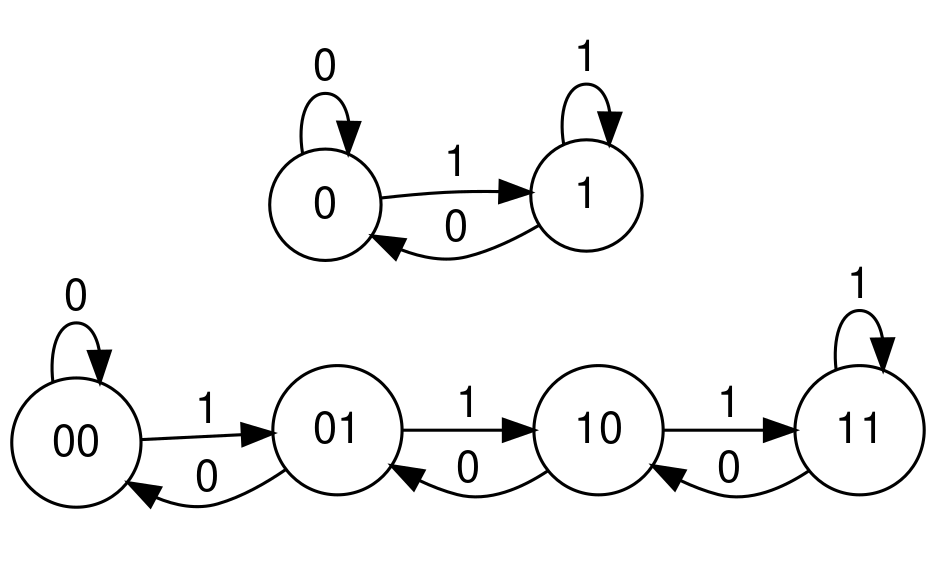
\includegraphics[width=10cm]{obrazky-figures/fsmpredictors.png}
  \caption{Schéma 1-bitového prediktoru (nahoře) a 2-bitového prediktoru (dole).
  Přechod do nového stavu se uskuteční při zpětné vazbě prediktoru. Přechod označený "1" znamená, že skok se doopravdy uskutečnil, přechod "0" znamená, že ke skoku nemělo dojít. }
  \label{fsmpredictor}
  % http://magjac.com/graphviz-visual-editor/
\end{figure}

% feedback, learning period
Dynamickým prediktorům je poskytována zpětná vazba v podobě informace o úspěšnosti poslední predikce.
V případě stavového automatu se stav posune po hraně značené "+", pokud byla predikce ověřena jako správná, nebo "-" v opačném případě.
Stavy prediktorů jsou inicializovány na určitou počáteční hodnotu.
První predikce mohou mít špatnou úspěšnost.
Tato fáze se nazývá učící období (learning period).
Po naučení vzoru se úspěšnost prediktoru ustálí.
Každý druh prediktoru je schopen naučit se pouze určitou podmnožinu vzorů.

% Adaptivní prediktor
% todo je ta historie globální, nebo pro instrukci?
Další variantou dynamických prediktorů je \emph{adaptivní prediktor}.
K predikci větvení jsou použity dvě informace: (1) historie posledních $k$ výsledků větvení dané instrukce a (2) záznam o chování skokové instrukce v minulých případech, kdy této instrukci předcházela stejná historie skoků.
Implementace spočívá v $k$ bitovém posuvném registru historie skoků a tabulce Pattern History Table (PHT): $2^k$ prediktorů pro každou instrukci.
Konkrétní prediktor je adresován vektorem historie a adresou instrukce. \cite{adaptiveBranch}

% todo Korelační prediktor
% adaptivní ale s globální historií
Korelační prediktor místo lokální historie používá jedinou, globální historií.

\subsection{Předpověď cílové adresy skoku}

% BTB, BTAC
K predikci cílové adresy skoků se využívá cache nazývaná Branch Target Buffer (BTB).
Tato tabulka se indexuje adresou skokové instrukce.

% komplikace s call - RSB
Komplikací jsou nepřímé skokové instrukce, neboli instrukce, jejichž cíl skoku není konstantní.
Takové skoky jsou využívány hlavně při návratu z funkce (\texttt{ret}), nebo při práci s ukazateli na funkce.
Predikce by byla nepřesná, protože funkce bývá volána z několika míst.
Úspěšnost lze zlepšit zásobníkem Return Stack Buffer (RSB), na který se při vstupu do funkce adresy ukládají a při opouštění vybírají.

% loop counter?

\chapter{Architektura RISC-V}
% todo ABI

RISC-V je otevřená instrukční sada architektury RISC.
Původně byla vyvinuta na UC Berkeley pro výukové účely.
Instrukční sada je navržena pro maximální jednoduchost a rozšiřitelnost, s cílem mít malé požadavky na hardware implementace.
\cite{riscvspec}

Definuje registry, samotnou instrukční sadu, její kódování a rozšíření, konvenci volání (ABI), výjimky.

Paměťový systém je navržen jako liitle-endian.
Specifikace připouští varianty s big-endian nebo oba systémy současně.

% general-purpose register computer
% Type Register-register (0, 3) - 0 memory operands, max 3 alu operands (one output)
% register, immediate, displacement addressing

\section{Architektura RISC}
% RISC a CISC

Architektury RISC (\emph{Reduced Instruction Set Computer}) kladou důraz na jednoduchost hardwaru, který instrukční sadu implementuje a na malou spotřebu energie.
Díky důrazu na nízkou cenu, malé ploše čipu a malému příkonu se často objevuje v malých zařízeních poháněných bateriemi, například v IoT a mobilních telefonech.

RISC se vyznačuje menším počtem instrukčních slov.
Typicky se jedná o minimální množinu instrukcí, ve které je možné popsat výpočty a práci s hardwarem.
Do instrukční sady se dostávají i další instrukce\footnote{Zajímavostí je instrukce \href{https://developer.arm.com/documentation/dui0801/h/A64-Floating-point-Instructions/FJCVTZS}{FJCVTZS} instrukční sady ARM. Jde o instrukci pro specifický převod čísla float64 na celé číslo. Tento výpočet je možné provést kombinací jiných instrukcí. Důvodem přidání této složitější instrukce do instrukční sady navzdory filozofii RISC byl výkon v důležitém případu užití -- tuto konverzi často provádějí interprety JavaScriptu.}, často z důvodu výkonu.
% https://stackoverflow.com/questions/50966676/why-do-arm-chips-have-an-instruction-with-javascript-in-the-name-fjcvtzs
% https://community.arm.com/arm-community-blogs/b/architectures-and-processors-blog/posts/armv8-a-architecture-2016-additions#:~:text=number%20signed%20addition-,Improved%20Javascript%20data%20type%20conversion,-Javascript%20uses%20the

Situace s menším množstvím instrukcí se dá vylepšit makry v assembleru, takzvanými \emph{pseudoinstrukcemi}.
Pseudoinstrukce jsou lexikální náhradou za instrukce s bližším sémantickým významem.
Tabulka \ref{table:pseudoins} uvádí několik příkladů.
Instrukční sadu je možné tímto způsobem virtuálně rozšířit.
V současném stavu, kdy je naprostá většina strojového kódu generována překladači, ale programátorský komfort není menší instrukční sadou negativně ovlivněn.

\begin{table}[ht]
\centering
\caption{Příklady pseudoinstrukcí a jejich odpovídajících reálných instrukcí. Pseudoinstrukce lépe vyjadřují význam operace, zároveň nijak nezatěžují hardware. Často obsahují implicitní argument.}
\begin{tabular}{|l|l|l|}
\hline
Pseudoinstrukce    & Ekvivalent z instrukční sady & Význam                         \\ \hline\hline
mv rd, rs          & addi rd, rs, 0     & Kopírování hodnoty             \\ \hline
neg rd, rs         & sub rd, x0, rs     & Negace celého čísla            \\ \hline
bgt rs, rt, offset & blt rt, rs, offset & Skok, pokud rs\textgreater{}rt \\ \hline
\end{tabular}
\label{table:pseudoins}
\end{table}

Kódování instrukcí je optimalizováno pro jednoduché načítání a dekódování.
Kódování mívá fixní délkou (např. 4\,B), operační kód a operandy jsou zapsány na předvídatelných místech v kódu.
Jednodušší dekódování znamená, že k jeho implementaci je zapotřebí méně hardwarových obvodů a čip má menší spotřebu.

Protipólem je architektura CISC (\emph{Complex Instruction Set Computer}), která definuje větší množství instrukcí.
Jedna instrukce může představovat i složitější operace, například aritmetickou operaci a načtení z paměti. Kódy mají typicky proměnlivou délku kódování.
Častěji používané operace mají kratší kódy, což se může projevit kompaktnější reprezentací programu v paměti.

Některé implementace CISC v rámci fáze dekódování převádí instrukce na sekvenci \emph{mikro-instrukcí}, další části linky dále operují s touto reprezentací.
Mikro-instrukce více připomínají instrukční sadu RISC.
Dekódování je složitější a proto má větší nároky na hardware.

\section{Instrukční sada}

Specifikace definuje základní celočíselnou sadu instrukcí ve dvou šířkách registrů, 32 bitů (\texttt{RV32I}) a 64 bitů (\texttt{RV64I}).
Verze \texttt{RV64I} je analogická s \texttt{RV32I}, s tím rozdílem, že registry mají šířku 64 bitů.
Procesor musí implementovat alespoň jednu z těchto dvou sad a libovolné množství rozšíření.
Dále budu popisovat pouze 32-bitovou variantu.

Z pohledu programátora je stav procesoru vyjádřen 31 obecnými registry pojmenovanými \texttt{x1}-\texttt{x31} a speciálními registry \texttt{x0} a \texttt{pc}.
Registr \texttt{x0} obsahuje konstantní hodnotu 0, registr \texttt{pc} obsahuje ukazatel na aktuální instrukci.

Základní instrukční sada definuje aritmetické instrukce, řídící instrukce a instrukce pro práci s pamětí.
Aritmetické instrukce nevyvolávají výjimky a nekontrolují přetečení.
Přetečení je možné zkontrolovat explicitní podmínkou.
Kódování instrukcí dovoluje vyjádřit přímé hodnoty v rozsahu 12 bitů.
Načtení 32 bitové konstanty je nutné provést kombinací instrukcí \texttt{LUI} a \texttt{ADDI}.

Skokové instrukce umožňují podmíněné a nepodmíněné relativní skoky.
Skok na absolutní adresu je možný kombinací instrukcí \texttt{LUI} a \texttt{JALR}.
Instrukce musí být zarovnané, proto skok na nezarovnanou adresu vyvolá výjimku.
Uložení návratové adresy provádí instrukce \texttt{JAL}.
Instrukce pro podmíněné skoky provádějí komparaci dvou registrů, vykonávají tedy dvě operace -- \emph{compare} a \emph{branch}.
% https://github.com/emb-riscv/specs-markdown/blob/develop/exceptions-and-interrupts.md#exceptions

Reprezentace instrukce v paměti zabírá 4 bajty, je zarovnaná na 4 bajty a je zakódována v jednom ze čtyř formátů\footnote{Rozšíření C navíc definuje komprimované 16-bitové instrukce}.
Formáty mají společné pole pro \emph{opcode} a 5-bitové adresy operandů-registrů.
Liší se ve využití zbylého prostoru, který je interpretován buď jako přímá hodnota, nebo další část \emph{opcode}.

% privileged specs
Specifikace RISC-V je rozdělena na dvě části.
Druhá část definuje privilegovaný režim, který je nutný k provozu operačního systému.
Architektura poskytuje tři režimy: Machine (M), Supervisor (S) a User (U).

Speciální registry (\emph{control and status registers} -- CSR) slouží ke sběru statistik a ladění.
Jejich čtení a nastavování je umožněno speciálními systémovými instrukcemi.
Jejich zápis je také vyvolán jako vedlejší efekt vykonávání instrukcí.
Instrukce \texttt{ECALL} slouží k žádosti o obsloužení jádrem.
Obdobně jako instrukce \texttt{SYSCALL} z ISA x86, argumenty jsou definovány podle používaného ABI.

\subsection{Rozšíření instrukční sady}
% rozšíření
Důležitou vlastností RISC-V je rozšiřitelnost.
Jednodušší čipy mohou implementovat pouze ta rozšíření, která ke svému účelu nutně potřebují.
Případně mohou jednoduše specifikovat vlastní instrukce relevantní pro svou doménu.

% genreal IMAFD
Rozšíření implementovaná daným zařízením jsou specifikována základní sadou a výčtem rozšíření.
Typickou sadu rozšíření vyjadřuje zkratka \texttt{RV32IMAFD}, také nazývanou \texttt{RV32G}.
Významy těchto rozšíření jsou uvedeny v tabulce \ref{table:extensions}.

\begin{table}[ht]
\centering
\caption{Nejvýznamnější rozšíření instrukční sady RISC-V. Celý výčet je k dispozici ve specifikaci RISC-V \cite{riscvspec}.}
\begin{tabular}{|c|l|}
\hline
Zkratka  & Popis rozšíření             \\ \hline\hline
M          & Celočíselné násobení a dělení     \\ \hline
A         & Atomické instrukce     \\ \hline
F         & podpora čísel \emph{single} podle standardu IEEE 754-2008\footnote{ANSI/IEEE Std 754-2008, IEEE standard for floating-point arithmetic, 2008.}     \\ \hline
D         & podpora čísel \emph{double} podle standardu IEEE 754-2008     \\ \hline
\end{tabular}
\label{table:extensions}
\end{table}

% výčet rozšíření

RV32E je varianta základní instrukční sady, která má pouze 16 obecných registrů.
Je určena pro čipy s velmi malou plochou.

\section{Paměťový model, vlákna}

RISC-V definuje 32-bitový paměťový prostor.
Přístupy do paměti nemusí být zarovnané, ale nezarovnané přístupy nemusí být atomické.

% RISC-V uses a memory model called “RVWMO” (RISC-V Weak Memory Ordering)
RISC-V používá paměťový model "RVWMO" (\emph{RISC-V Weak Memory Ordering}).
V tomto modelu může jádro pozorovat paměťové instrukce jiného jádra v jiném než původním pořadí.

% FENCE synchronisation, chapter 6 of manual
% todo je toto faktuální?
Pro komunikaci vláken prostřednictvím sdílené paměti musí proto být zavedena synchronizace.
Rozšíření A k tomuto účelu představuje instrukce pro atomické paměťové operace.
Instrukce \texttt{FENCE} umožňuje realizovat paměťovou bariéru a tím vynutit pořadí paměťových operací.

% todo komunikace s memory mapped i/o

\section{Aplikační binární rozhraní}
% https://github.com/riscv-non-isa/riscv-elf-psabi-doc/blob/master/riscv-abi.adoc

Aplikační binární rozhraní definuje konvenci volání a specifika RISC-V pro formáty ELF a DWARF.
Předepisuje také velikosti a zarovnání pro datové typy jazyka C.
\cite{riscvabi}

Konvence volání označuje způsob komunikace vstupů a výstupů mezi procedurami.
Při popisu se používají aliasy pro jména registrů.
Tato jména odrážejí funkci registru v konvenci volání.
Například registr \texttt{x2} se také nazývá \texttt{sp} (stack pointer), jelikož ukazuje na vrchol zásobníku.
Pro každý registr je specifikováno, zda má volání procedury zachovat jeho hodnotu, nebo je možné ji přepsat.

RISC-V ABI preferuje předávání argumentů registry.
Celočíselné argumenty se předávají registry \texttt{a0}-\texttt{a7}.
Pro čísla s plovoucí desetinnou čárkou se používají registry \texttt{fa0}-\texttt{fa7}.
Pokud počet registrů nestačí, další argumenty se předávají \emph{zásobníkem}.

%
% Webová rozhraní
%

\chapter{Webová rozhraní}
% Significance of Web Development

Webový prohlížeč a webové technologie se v posledních letech staly uživateli očekávaným standardem pro interakci s počítačem.
Pokud aplikace dokáže splnit své požadavky v prostředí prohlížeče, potom je pro vývojáře výchozí volbou.
Hlavním důvodem popularity je ten, že uživatelé mohou začít aplikaci okamžitě používat.
Vývoj webové aplikace je také rychlejší a levnější.
% nemuzu najit source

% v posledních letech se hranice začínají ztrácet. Mnoho desktopových aplikací je implementováno za pomoci webových technologií.

S rostoucí popularitou, implementací nových standardů a vývojem rámcových řešení podíl webových aplikací stále roste.
% https://survey.stackoverflow.co/2023/#technology  ??

\section{Základní koncepty a technologie}
% browser, HTTP, HTML, CSS, JS, React
% Frontend vs Backend
% frameworky, bundling, polyfills

Základem obsahu na World Wide Web jsou \emph{hypermédia}.
Hypermediální dokumenty jsou spojeny navigovatelnými referencemi, takzvanými \emph{hyperlinky}.
Společně tvoří síť propojených informací, kde uživatelé mohou pohodlně přecházet mezi jednotlivými stránkami a získávat různorodý obsah, například ve formě textu nebo videa.
Dokumenty mohou být interaktivní -- tímto způsobem jsou implementovány složitější webové aplikace.

Dokumenty, jejich reprezentace a způsob jejich renderování jsou definovány kolekcí standardů vyvinutých WHATWG. Hlavním standardem je HTML Standard, který definuje jazyk HTML a některá API jako například \texttt{localStorage}.
Standard se dále odkazuje na velké množství dalších standardů, např. HTTP, CSS, Unicode, XML a standardy obrazových formátů. \cite{htmlStandard}
% Cascading Style Sheets Level 2 Revision 2, B. Bos, T. Çelik, I. Hickson, H. Lie. W3C.
% Hypertext Transfer Protocol (HTTP/1.1): Message Syntax and Routing, R. Fielding, J. Reschke. IETF.

Tyto standardy jsou implementovány webovými prohlížeči.
Prohlížeč má roli hypermediálního klienta.
Jeho prvním úkolem je komunikovat se servery v síťové architektuře klient-server, ve které klienti poptávají zdroje od speciálních účastníků sítě -- serverů.
Zdroji jsou v případě webu myšleny hypertextové dokumenty, multimédia a další soubory.
Komunikace mezi uzly je rozvedena v následující sekci.

Druhým úkolem prohlížeče je tyto dokumenty zobrazovat uživateli.
Uživatelská rozhraní blíže rozvedu v sekci \ref{ui_scripting}.

\subsection{Přenosové protokoly}
% main concepts of HTTP

Výměna dokumentů mezi serverem a klientem probíhá bezstavovým textovým protokolem HTTP.
Tento protokol aplikační vrstvy je postaven na TCP, poskytuje tedy spolehlivý přenos.
Jedná se o protokol typu request/response.

Zdroje jsou na webu identifikované pomocí \emph{Uniform Resource Identifier} (URI).
V hlavičce zprávy typu request se přenáší verze protokolu, metoda, URI požadovaného zdroje, hlavičky s informacemi o klientovi a požadovaném zdroji a v některých případech i tělo zprávy s libovolnou sekvencí bajtů.
\cite{http-rfc}

Server odpovídá zprávou response, která obsahuje statusový kód, hlavičky a data určitého typu.

HTTP poskytuje několik sémantických metod.
Metody \texttt{GET} a \texttt{HEAD} slouží k získání dokumentů.
Metodami \texttt{DELETE}, \texttt{POST} a \texttt{PUT} klient žádá server o provedení nějakého \emph{vedlejšího efektu}, například přidání nového příspěvku na sociální síť.

Trojciferný statusový kód odpovědi indikuje, zda byl příspěvek zpracován.
Konkrétní kódy mají specifické významy, dělí se do pěti skupin: informační, úspěchové, přesměrovací, chybové na straně klienta a chybové na straně serveru.

% QUIC
S vyvíjejícími se požadavky na web se protokol HTTP vyvíjel do verze 2 a 3.
Firma Google vyvinula vlastní protokol QUIC, který především snižuje marži šifrované komunikace a umožňuje použít jedno spojení k přenosu několika streamů (multiplexing).
Vyšší efektivita přenosu se pozitivně projevuje především při používání na pomalejších mobilních sítích.

% todo Time to First Byte (TTFB)

\subsubsection{Sezení}

HTTP je bezstavovým protokolem, aplikace ale může pro své cíle vyžadovat kontext.
Příkladem kontextu může být identita uživatele pro autorizaci nebo personalizaci.

% cookies
Mechanismus cookies slouží ke komunikaci kontextu při dotazu.
Cookie je textový token vytvořený serverem, přenášený v hlavičce každého dotazu.
Cookies jsou typicky využity k ustanovení sezení (\emph{session}) -- sekvence dotazů sdílející kontext. 
Konkrétní způsob jejich využití závisí na serveru.
\cite{cookies}

Jedním ze schémat k ustanovení spojení je identifikátor sezení -- \emph{session ID}.
Na straně serveru je tento identifikátor spojen s konkrétními daty v databázi sezení.

Druhým častým způsobem navázání sezení je technologie JSON Web Token (JWT).
Tento token obsahuje libovolná textová data a datum expirace.
Token je kryptograficky podepsán, aby byla zaručena integrita dat.

\subsubsection{Zabezpečení}

% TLS
Protokol HTTP neposkytuje důvěrnost ani integritu.
Pokud je aplikace vyžaduje, je potřeba navázat spojení přes protokol HTTPS.
HTTPS je protokol HTTP přenášený pomocí kryptografického protokolu \emph{Transport Layer Security} (TLS).

Protokol spočívá v ustanovení symetrického klíče sezení.
Identita serveru je také ověřena u důvěřované certifikační autority.

Ustanovení TLS (verze 1.2) spojení přidává latenci 2 RTT (Round Trip Time).
S navázáním TCP spojení a samotným HTTP dotazem se vytvoření nového spojení dostává na minimální zpoždění 4 RTT (není započítáno vyhledání v DNS).
Takové zpoždění se může významně negativně projevit dlouhou čekací dobou na načtení stránky, obzvlášť na mobilních sítích.
TLS verze 1.3 přináší schopnost obnovit spojení na dříve navštívenou stránku za 2 RTT díky funkcionalitě 0-RTT. \cite{tls}
% https://blog.cloudflare.com/introducing-0-rtt

% mitm

% session stealing
Hodnoty cookies jsou přenášeny v hlavičkách HTTP, nešifrovaně.
RFC 6265 \cite{cookies} doporučuje, aby byly citlivé hodnoty šifrovány a podepsány, a to i v případě, že je hlavička přenášena přes HTTPS.

\section{Skriptování}
\label{ui_scripting}

Interaktivitu uživatelských rozhraní pohání skriptovací jazyk JavaScript.
Skriptům jsou přístupná API pro manipulaci DOM (Document Object Model), což je stromová reprezentace aktuálního dokumentu.

% Použití
Skriptování se používá k vytváření dynamických a interaktivních webových rozhraní, validaci a zasílání formulářů a prací s různými API.
Webová API například umožňují skriptům pracovat se souborovým systémem, nebo komunikovat pomocí HTTP.

Příklady použití API k manipulaci DOM jsou volání jako \texttt{element.appendChild}, nebo \texttt{querySelector}.
Při vývoji složitých aplikací se ale typicky tato volání nepoužívají přímo, ale abstrahovaně, prostřednictvím knihoven.
Mezi nejznámější patří React, Angular, a Vue.js.

V současné době je rozvíjena technologie WASM, což je virtuální stroj založený na bajtkódu.
Tato technologie umožňuje psát programy pro web v libovolném kompilovaném programovacím jazyce a slibuje vyšší výkon.
Technologie je však stále v zárodku, proto ji v této práci podrobněji nepopíšu. 

\subsection{React}

React je open-source\footnote{\href{https://github.com/facebook/react}{https://github.com/facebook/react}} knihovna vyvinutá firmou Meta pro vytváření uživatelských rozhraní.

Základním stavebním blokem UI je \emph{komponent}.
Každá jednotlivá stránka se skládá ze stromové hierarchie komponentů.

Komponent je uzavřený celek s definovaným programovým rozhraním, který implementuje jeden prvek uživatelského rozhraní včetně jeho chování a vzhledu.
Vývoj aplikace orientovaný na komponenty podporuje znovupoužitelnost, modularitu a testovatelnost.
Komponenty mohou mít vlastní vnitřní stav a vykonávat kód v různých stádiích životního cyklu (změna parametrů, zánik instance komponentu apod.).

React k definici komponentů používá rozšíření syntaxe JavaScriptu nazývané JSX.
Díky JSX je možné vkládat fragmenty HTML přímo do skriptů.
Příklad jednoduchého komponentu je uveden v příkladu \ref{jsx}.
Soubory \texttt{.jsx} je nutné zkompilovat do standardního JavaScriptu. 

\begin{figure}[hbtp]
    \begin{lstlisting}[]
export default function List({items}) {
  const listItems = items.map(item =>
    <li key={item.id}>
        <b>{item.text}</b>
    </li>
  );
  return <ul className="large-font">{listItems}</ul>;
}
    \end{lstlisting}
    \caption{Příklad komponentu definovaného v \texttt{.jsx} souboru. Komponent renderuje array předanou v parametrech jako list v HTML. Komponent definuje jak logiku, tak i vzhled. S fragmenty HTML je možné pracovat jako s hodnotami.}
    \label{jsx}
\end{figure}

Knihovna je velmi populární, díky tomu lze v projektech využít velkého množství dalších knihoven (například pro práci s globálním stavem), nebo využít celé předpřipravené komponenty.

Nevýhodou je výkon aplikací oproti řešení v čistém JavaScriptu a velikost knihovny, kterou je nutné stáhnout při návštěvě stránky (~130\,kB kódu).
% todo cite?

V současné době je doporučováno React používat prostřednictvím jiného rámcového řešení, jakým je například \emph{Next.js}.

\subsection{Next.js}

Next.js je \emph{fullstackovým frameworkem}.
Znamená to, že výsledná aplikace zastává funkci serveru i klienta.
Tento framework doplňuje React do uceleného řešení webové aplikace.

% server
Next.js poskytuje implementaci serveru.
Dostupné cesty stránek jsou definovány strukturou souborů (file-system based router).
Je podporováno i dynamické směrování.

Next.js používá hybridní přístup k renderování.
Stránky jsou pokud možno alespoň částečně staticky renderované na serveru.
Pokud stránka obsahuje dynamický obsah, je dodatečně renderovaný na straně klienta.
Po přijetí statické stránky je \emph{hydratována}, čímž se stává interaktivní.
Pouze první stránka je stažena ze serveru -- následující navigace jsou vykonány JavaScriptem.

% optimizations
Framework se stará o cachování, přednačítání zdrojů a další optimalizace s cílem zvýšit výkon aplikací.
Významně zjednodušuje nasazení aplikace do provozu.

% todo

\section{Uživatelská rozhraní}

% User Experience of Web Browsing - The Relationship of Usability and Quality of Experience
% citace se mi moc nehodí

% IS0 DIS 9241-11 -- usability definition
\emph{Uživatelská rozhraní} (User Interface -- UI) se převážně zaměřují na aspekt použitelnosti -- efektivitu a spokojenost, s jakou je uživatel schopen dosáhnout svých cílů.
Celková příjemnost produktu ale může záviset na více faktorech, než pouze použitelnost.
Pokud se návrh aplikace zaměří pouze na použitelnost, celkový dojem z aplikace nemusí být optimální. 
\cite{pleasureInProduct}

Použitelnost je ovlivněna mnoha faktory, například intuitivnost, spolehlivost, nebo úsilí nutné k používání aplikace.

Estetická příjemnost, uspořádanost a čitelnost rozhraní jsou také důležitými faktory pro jejich pozitivní vnímání. \cite{webAesthetics}

\subsection{Použitelnost}

Použitelnost je vlastnost systému vyjadřující jeho jednoduchost pro používání i naučení.

% https://www.nngroup.com/articles/cognitive-walkthroughs
% todo překlad Cognitive walkthrough ??
Jedním ze způsobů evaluace použitelnosti je kognitivní analýza (\emph{Cognitive walkthrough}).
Tato metoda se zaměřuje na nejdůležitější úkoly v aplikaci a jednotlivé kroky, ze kterých se úkol skládá.
Analýza probíhá z perspektivy nového uživatele a jeho schopnosti dosáhnout svých cílů používáním aplikace.
Metodu je možné začít využívat již v raných fázích vývoje, jakmile je k dispozici prototyp.
\cite{cognitiveWalkthrough}

% Postup
Vyhodnocení vykonávají specialisté (vývojáři a odborníci na danou doménu).
Postupně jsou analyzovány jednotlivé úkoly z předem definovaného seznamu.
Jeden z účastníků provádí vybraný úkol a zastavuje se při každém kroku.
Ostatní účastníci debatují o potenciálu uživatele úspěšně krok provést.
K hodnocení jim pomáhají předem připravené otázky.

Výstupem analýzy je seznam prvků rozhraní, které mohou být pro nové uživatele představovat překážky.

\subsection{Dostupnost}
% accesibility
% screen readers
% https://en.wikipedia.org/wiki/Web_Content_Accessibility_Guidelines

Dostupnost v kontextu webu se zaměřuje na podporu široké škály možností interakce s webovými aplikacemi.
Důležitou skupinou jsou invalidní uživatelé a uživatelé mobilních zařízení.
Standardizační organizace World Wide Web Consortium (W3C) vydává směrnice \emph{Web Content Accessibility Guidelines}\footnote{\href{https://www.w3.org/WAI/standards-guidelines/wcag/}{https://www.w3.org/WAI/standards-guidelines/wcag/}} určené pro vývoj dostupných aplikací.

Velká část implementace dostupnosti spočívá v anotaci obsahu tak, aby byl lépe strojově zpracovatelný.
Příkladem může být význam vstupních polí, správné použití sémantických HTML značek, nebo textové alternativy k obrazovým datům.

Prezentace by se měla adaptovat na různá rozlišení a orientaci obrazovky.
Měla by mít dostatečný kontrast textu a pozadí.

Důležité je také možnost ovládat celou aplikaci pomocí klávesnice.

Kvalitní knihovny pro prvky uživatelského rozhraní jsou navrženy v souladu se standardy a mohou zajistit lepší dostupnost bez nutnosti investovat značné množství zdrojů do vyvinutí vlastního řešení.
% Jak se accessibility vyvíjí: https://webaim.org/projects/million/#aria

Accessible Rich Internet Applications (ARIA) je skupina atributů, kterými lze sémanticky anotovat HTML značky.
Atribut \texttt{role} u značky vyjadřuje jeho roli v rozhraní a používá se v situacích, ve kterých nelze použít vhodnou sémantickou značku.
Role elementu může být strukturní (\texttt{tooltip}, \texttt{note}), widget (\texttt{searchbox}, \texttt{slider}) a další.

\subsection{Měření uživatelského zážitku}
%  "uživatelský zážitek" nebo "uživatelský komfort"

Měření uživatelského zážitku ve webových aplikacích je klíčovým prvkem moderního návrhu a vývoje aplikací.
Pro vytvoření dobrého rozhraní je nezbytné porozumět tomu, jak uživatelé vnímají a využívají webové aplikace.
Uživatelský zážitek (UX -- User Experience) zahrnuje vizuální dojem, snadnost navigace, efektivitu úkonů a celkovou přívětivost rozhraní.
Měření těchto aspektů pomáhá vývojářům identifikovat potenciální problémy a optimalizovat užitečnost aplikace.

Uživatelé vnímají vizuální odezvu jako okamžitou, pokud se odehraje do 30\,ms.
Vnímaná kvalita významně klesá, pokud je odezva vyšší než 100\,ms. \cite{interactivityDelay}

% flow, immersion

\subsubsection{Kvalitativní metody}
% interviews
% User Testing, Session Analysis, A/B

Vnímání produktu jeho uživatelem je velmi subjektivní.

Poskytnutí formuláře nebo dotazníku pro zpětnou vazbu je nejjednodušší způsob implementace sběru dat od uživatelů.
Má ale zásadní nevýhodu -- uživatel musí věnovat vlastní čas a úsilí k poskytnutí zpětné vazby.
Důsledkem je, že jsou hlášeny pouze problémy, které si uživatel uvědomuje, dokáže popsat a jsou pro něj dostatečně důležité.
Navíc uživateli musí záležet na tom, aby byl nedostatek opraven.

Uživatelská přívětivost je měřitelná analýzou sezení.
Metoda Real user monitoring (RUM) instrumentuje aplikaci a tvoří záznam akcí v čase.
Poznatky o nedostatcích lze získat pasivním porovnáním akcí úspěšných a neúspěšných uživatelů.
% https://en.wikipedia.org/wiki/Real_user_monitoring

% focus groups, interviews

\subsubsection{Kvantitativní metody}
\label{kvantMethods}
% Cumulative Layout Shift (CLS)
% Time to Interactive (TTI)
% Largest Contentful Paint (LCP)
% Page Load Time (PLT) or Speed Index (SI)
% Interaction to Next Paint (INP)

% https://support.google.com/webmasters/answer/9205520?hl=en

\emph{Web Vitals} je soubor metrik vyjadřujících kvalitu uživatelského zážitku z pohledu rychlosti načítání a výkonu při interakci.
Metriky odrážejí architekturu aplikace i infrastrukturu, na které je aplikace nasazena.

\emph{Largest Contentful Paint} (LCP) měří dobu od navigace na stránku do zobrazení největšího prvku UI.
Tento čas zahrnuje dobu sestavení spojení.
Za dobrý výsledek se považuje hodnota menší než 2,5\,s.

\emph{Cumulative Layout Shift} (CLS) měří míru neočekávaných změn pozic prvků rozhraní.
Tyto posuny jsou způsobeny postupným načítáním obsahu (typicky obrázků, reklam a jiného dynamického obsahu).
Velká nestabilita rozvržení stránky způsobuje frustraci uživatele a možnost kliknout na nechtěný prvek rozhraní.

\emph{Interaction to Next Paint} (INP) měří responzivitu aplikace jako dobu mezi interakcí a prezentací dalšího vyrenderované obrazovky.
Za dobrou hodnotu se považuje 200\,ms.
Některé akce přirozeně trvají delší dobu.
V takovém případě je nutné prezentovat zpětnou vazbu, aby uživatel nenabyl dojmu, že aplikace přestala odpovídat. 

Další měřené metriky zahrnují \emph{Time to First Byte} (TTFB), nebo \emph{First Contentful Paint} (FCP).

Vyhledávače tyto metriky využívají k odhadu kvality webové stránky a její upřednostnění ve výsledcích, což může být důležité pro dosažení cílů organizace.
Výsledky měření mají určitou distribuci hodnot podle výkonu zařízení a kvality internetového spojení se serverem.
Je doporučeno pracovat se 75. percentilem hodnot metrik.

\cite{coreWebVitals}

% number of clicks to finish a task
% load times

\section{Architektura systému}
% Aplikační rozhraní
% https://htmx.org/essays/hypermedia-apis-vs-data-apis/

V architektuře webových aplikací se klíčově uplatňuje model klient-server, v rámci kterého klient (webový prohlížeč) a server komunikují přes standardizované protokoly.
Dva základní přístupy ke komunikaci jsou hypermediální API a datová API.

Hypermediální API je rozhraní, které poskytuje hypermédia.
Typicky se jedná o dokumenty nebo části dokumentu v jazyce HTML, obrázky a videa ve formátech přímo podporovaných prohlížeči.
Tyto odpovědi jsou přímo zobrazovány klientem.
Jedná se o původní přístup poskytování dat v kontextu webových aplikací.
Příkladem jsou statické HTTP servery, nebo servery renderující HTML při dotazu (\emph{Server-Side Rendering}) využívající knihovny jako například Django, Express a Ruby on Rails.

Oproti tomu datové API poskytuje strukturovaná data, která nejsou určena k přímému zobrazení.
Prvotní stažení stránky stále proběhne v podobě HTML. 
Součástí stránky je ale JavaScriptový kód, který dál pracuje s datovým API.
Data jsou zpracovávána do nového stavu DOM, který je prohlížečem prezentován uživateli.
% SPA/MPA

% globální stav 
% mvc? :(

\subsection{Globální stav aplikace}

Globální stav jsou data dostupná ze všech částí aplikace.
Využívá se ke zpřístupnění dat, se kterými pracuje velká část aplikace a ke sdílení dat mezi moduly.
Příklady globálně ukládaných informací jsou data o sezení, uživatelská data a konfigurace aplikace. 

Dříve zmíněná knihovna React podporuje práci s globálním stavem ve formě \texttt{Context API}.
Vytvořený \emph{kontext} je zpřístupněn všem komponentům hlouběji ve stromu.

% https://blog.isquaredsoftware.com/2017/05/idiomatic-redux-tao-of-redux-part-1/
\emph{Redux} je zástupcem knihoven pro správu stavu.
Stav je zde reprezentován jediným objektem, který je možné libovolně číst.
Změny globálního stavu jsou možné výhradně skrze \emph{akce} -- čisté funkce transformující daný stav do nového stavu.
Redux vybízí k centralizaci logiky aplikace v definici stavu jeho akcích.
% todo pure function překlad??

% perzistence, tools
Ekosystém nástrojů a knihoven ulehčuje vývoj aplikace.
Ladící konzole dovoluje prohlížení stavu, zaznamenává všechny změny stavu a umožňuje změny přehrát.
Jiné knihovny například ulehčují perzistenci stavu napříč sezeními.

\section{Vývojové praktiky}
% git, CI, deployment, packages
% git-flow?

Při vývoji webových aplikací je klíčové implementovat moderní vývojové praktiky, které zajišťují efektivní správu kódu, plynulý vývoj, komunikaci a nasazení aplikace do provozu.

Git, systém pro správu verzí kódu, hraje klíčovou roli ve sledování a dokumentování změn v kódu.
Hlavním konceptem gitu je \emph{commit}, záznam stavu kódu.
Každý commit je uzlem v grafu, hrany vyjadřují jejich následnost.
Události jako například vznik nového commitu, nebo schválení kódu mohou být spouštěčem pro automatizované testování a nasazení.

Continuous Integration a Continuous deployment (CI/CD) je dalším důležitým konceptem.
Díky CI probíhají automatizované akce, například sestavení projektu a testování, což zvyšuje jistotu, že nový kód dosahuje dobré kvality.
Jsou generována hlášení o výsledcích běhů.
Automatizace snižuje pravděpodobnost lidské chyby.

% Packages
Využití knihoven zrychluje vývoj, populární knihovny zároveň bývají robustní a dobře navržené.  
Manažer balíčků umožňuje velmi jednoduchou správu závislostí projektu.

\subsection{Nasazení}

Proces nasazování představuje klíčový okamžik v životním cyklu webové aplikace.
Automatizované postupy umožňují rychlé a konzistentní nasazení nových verzí na produkční nebo předprodukční server.
To nejen minimalizuje riziko lidských chyb, ale také šetří manuální úkony.

% Virtualizace
Častým problémem při nasazování aplikace na server bývají její požadavky na prostředí -- verze operačního systému, nainstalované programy, proměnné prostředí a další.
Systém Docker tento problém řeší tak, že celé prostředí popíše předpisem pro jeho vytvoření.
Při spuštění \emph{kontejneru} virtualizační vrstvou se tento předpis vykoná v izolovaném prostředí.

Výsledkem je předvídatelné nasazení převážně abstrahované od konkrétního systému.
Změna serveru, na kterém aplikace běží, představuje žádné nebo minimální změny v kódu nebo konfiguraci. 
% no musí být stejná architektura procesoru v určitých případech?

\subsection{Testování}

Robustní testovací řešení významně usnadňuje vývoj nových funkcí aplikace, stejně jako změny v existující funkcionalitě.

Existují různé druhy testování softwaru.
Každé se zaměřuje na určitou vrstvu softwarového produktu:
\begin{itemize}
    \item Testování na úrovni softwarových modulů (Unit Testing),
    \item Testování interakce modulů (Integration Testing) 
    \item Holistické testování (End-to-end testing)
\end{itemize}

Testování by mělo být automatizované.
Ponechání procházejících testů v projektu zabraňuje regresím.
Nevhodný návrh testů může mít za důsledek jejich přílišnou závislost na vnitřní implementaci.
Při změnách v implementaci takové testy vyžadují častou opravu, což ztěžuje údržbu.

Webové rozhraní lze testovat mnoha způsoby a má svá specifika.
Testy mohou ověřovat, zda se na stránce vyskytuje daný text a provést gramatickou kontrolu.
Testy pro dostupnost mohou kontrolovat kontrast textu a anotaci HTML značek.
Můžeme aplikovat kvantitativní metody (sekce \ref{kvantMethods}) a sbírat metriky od skutečných uživatelů.

Testování funkcí webových uživatelských rozhraní je často prováděno manuálně.
Rozhraní bývají složitá a jejich automatizace je velmi pracná na implementaci a údržbu. 
GUI by mělo být testováno ve více prohlížečích.
